\documentclass[12pt]{article}
\usepackage{graphicx}
\usepackage{subcaption}
\usepackage{geometry}
\usepackage{float}
\geometry{a4paper, portrait, margin=1in}


\title{DIC data for Surflex material}
\author{Sumeet Mishra \\ Department of Materials \\ University of Manchester}


\begin{document}
\maketitle

\section{Strain maps}

\subsection{Sample at 0 degrees}
\begin{figure}[H]
    \centering
    \begin{subfigure}[b]{0.31\textwidth}
        \includegraphics[width=\textwidth]{../0-1/strain_map_t_5}
    \end{subfigure}
    \begin{subfigure}[b]{0.31\textwidth}
        \includegraphics[width=\textwidth]{../0-1/strain_map_t_5}
    \end{subfigure}
    \begin{subfigure}[b]{0.31\textwidth}
        \includegraphics[width=\textwidth]{../0-1/strain_map_t_5}
    \end{subfigure}
\end{figure}


\subsection{Sample at 45 degrees}
\begin{figure}[H]
    \centering
    \begin{subfigure}[b]{0.31\textwidth}
        \includegraphics[width=\textwidth]{../45-1/strain_map_t_5}
    \end{subfigure}
    \begin{subfigure}[b]{0.31\textwidth}
        \includegraphics[width=\textwidth]{../45-1/strain_map_t_5}
    \end{subfigure}
    \begin{subfigure}[b]{0.31\textwidth}
        \includegraphics[width=\textwidth]{../45-1/strain_map_t_5}
    \end{subfigure}
\end{figure}

\subsection{Sample at 90 degrees}
\begin{figure}[H]
    \centering
    \begin{subfigure}[b]{0.31\textwidth}
        \includegraphics[width=\textwidth]{../90-1/strain_map_t_5}
    \end{subfigure}
    \begin{subfigure}[b]{0.31\textwidth}
        \includegraphics[width=\textwidth]{../90-1/strain_map_t_5}
    \end{subfigure}
    \begin{subfigure}[b]{0.31\textwidth}
        \includegraphics[width=\textwidth]{../90-1/strain_map_t_5}
    \end{subfigure}
\end{figure}

\section{Shape Change Maps}

\subsection{Sample at 0 degrees}
\begin{figure}[H]
    \centering
    \begin{subfigure}[b]{0.31\textwidth}
        \includegraphics[width=\textwidth]{../0-1/shape_change_t_5}
    \end{subfigure}
    \begin{subfigure}[b]{0.31\textwidth}
        \includegraphics[width=\textwidth]{../0-1/shape_change_t_5}
    \end{subfigure}
    \begin{subfigure}[b]{0.31\textwidth}
        \includegraphics[width=\textwidth]{../0-1/shape_change_t_5}
    \end{subfigure}
\end{figure}


\subsection{Sample at 45 degrees}
\begin{figure}[H]
    \centering
    \begin{subfigure}[b]{0.31\textwidth}
        \includegraphics[width=\textwidth]{../45-1/shape_change_t_5}
    \end{subfigure}
    \begin{subfigure}[b]{0.31\textwidth}
        \includegraphics[width=\textwidth]{../45-1/shape_change_t_5}
    \end{subfigure}
    \begin{subfigure}[b]{0.31\textwidth}
        \includegraphics[width=\textwidth]{../45-1/shape_change_t_5}
    \end{subfigure}
\end{figure}

\subsection{Sample at 90 degrees}
\begin{figure}[H]
    \centering
    \begin{subfigure}[b]{0.31\textwidth}
        \includegraphics[width=\textwidth]{../90-1/shape_change_t_5}
    \end{subfigure}
    \begin{subfigure}[b]{0.31\textwidth}
        \includegraphics[width=\textwidth]{../90-1/shape_change_t_5}
    \end{subfigure}
    \begin{subfigure}[b]{0.31\textwidth}
        \includegraphics[width=\textwidth]{../90-1/shape_change_t_5}
    \end{subfigure}
\end{figure}


\section{Longitudinal and transverse strain}


\begin{figure}[H]
  \centering
    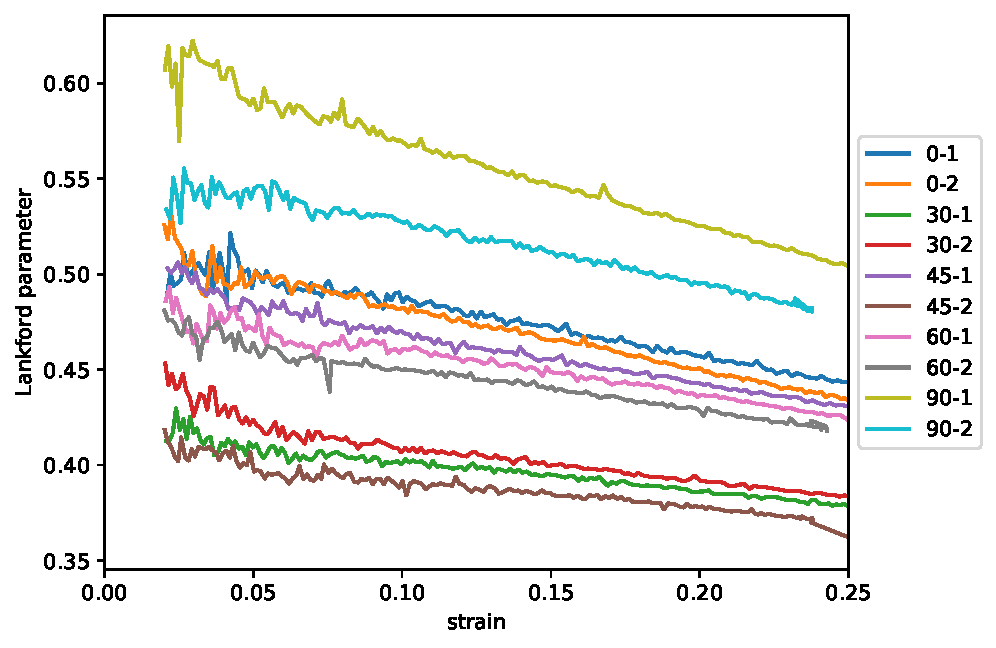
\includegraphics[width=0.5\textwidth]{../lankford_parameter}
\end{figure}

\section{Strain Ratio}

\begin{figure}[H]
  \centering
    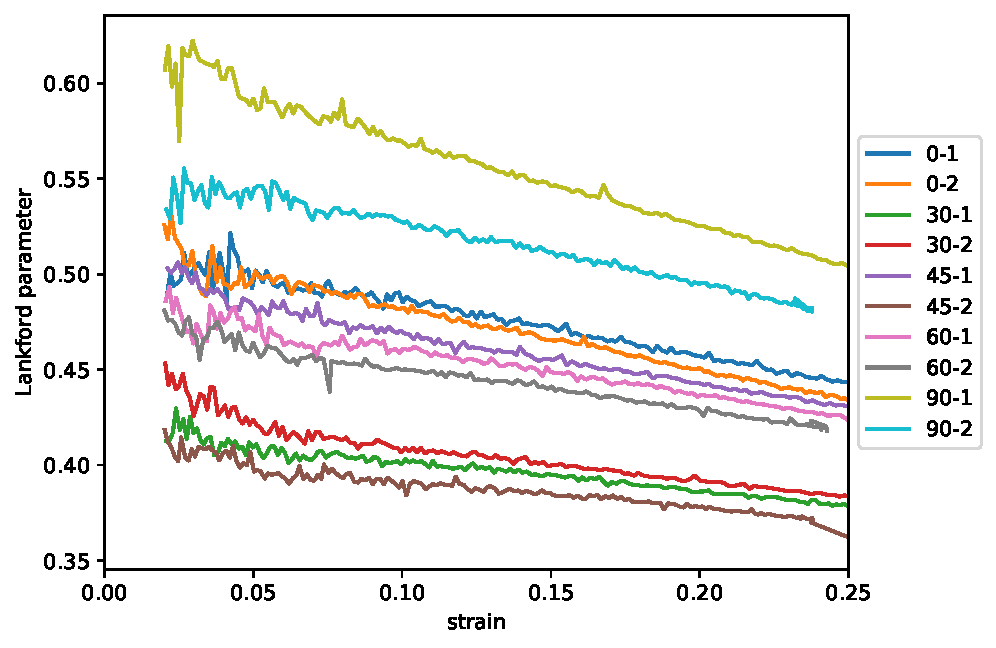
\includegraphics[width=0.5\textwidth]{../lankford_parameter}
\end{figure}


\section{Lankford parameter}

\begin{figure}[H]
  \centering
    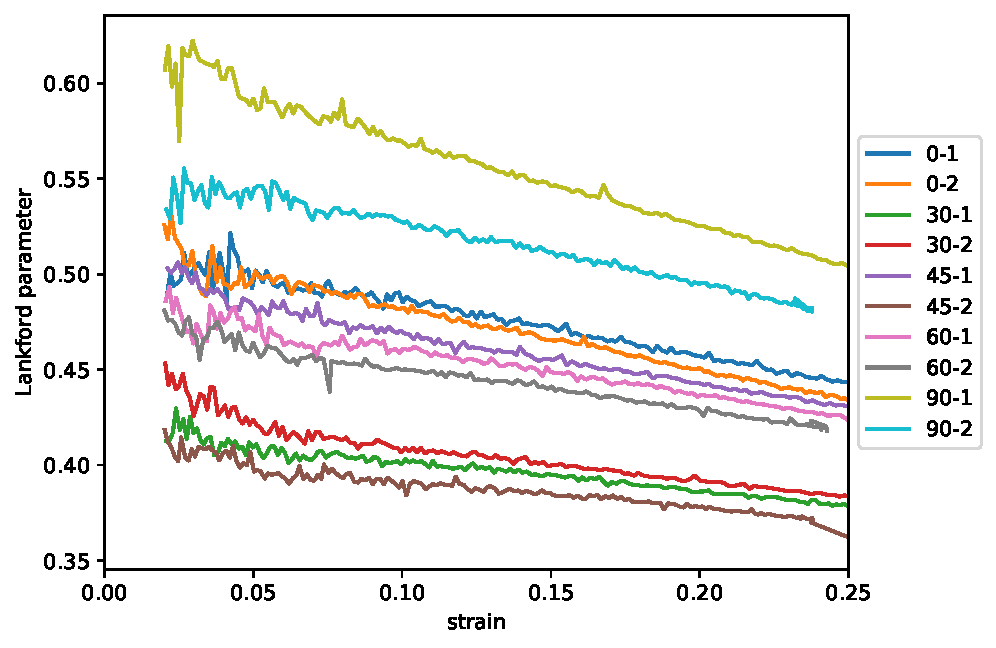
\includegraphics[width=0.5\textwidth]{../lankford_parameter}
\end{figure}



\end{document}


